\documentclass{beamer}

\mode<presentation>
{ \usetheme{Copenhagen} }

\AtBeginSection[]
{
   \begin{frame}
       \frametitle{Outline}
       \tableofcontents[currentsection]
   \end{frame}
}

\usepackage{graphicx}

\title{Git}
\author{Nelson Elhage\and Anders Kaseorg}
\institute{Student Information Processing Board}
\date{October 21, 2008}

\begin{document}

\begin{frame}
    \titlepage
\end{frame}

\section{The Git Model}

\begin{frame}
  \frametitle{The Git Model}

  \begin{itemize}
  \item A Git repository contains four kinds of \emph{objects}.
  \item An object is either a \emph{blob} (file), a \emph{tree}
    (directory), a \emph{commit}, or a \emph{tag}.
  \item Every object is uniquely identified by a 40 hex digit number,
    which is the SHA-1 hash of its contents.
    \begin{itemize}
    \item Don't worry---identifiers can be abbreviated by truncation,
      or referenced with human-readable names.
    \end{itemize}
  \item Some objects refer to other objects using their identifiers.
  \end{itemize}
\end{frame}

\begin{frame}
  \frametitle{Objects}

  \begin{itemize}
  \item A blob object is a file's contents.
  \item A tree object is a directory---a list of zero or more
    directory entries, each of which has
    \begin{itemize}
    \item a \emph{name}
    \item a UNIX \emph{mode}
    \item a tree id or blob id
    \end{itemize}
  \item A commit object contains
    \begin{itemize}
    \item a tree id
    \item zero or more \emph{parents}, which are commit ids
    \item an \emph{author} (name, email, date)
    \item a \emph{committer} (name, email, date)
    \item a \emph{log message}
    \end{itemize}
  \item A tag object contains
    \begin{itemize}
    \item a \emph{tag name}
    \item a \emph{tagger} (name, email, date)
    \item a reference to another object (usually a commit)
    \item an optional \emph{log message}
    \end{itemize}
  \end{itemize}
\end{frame}

\begin{frame}
  \frametitle{A commit}
  \hspace*{-0.5cm}\includegraphics[width=12cm]{commit}
\end{frame}

\begin{frame}
  \frametitle{More commits}
  \hspace*{-0.5cm}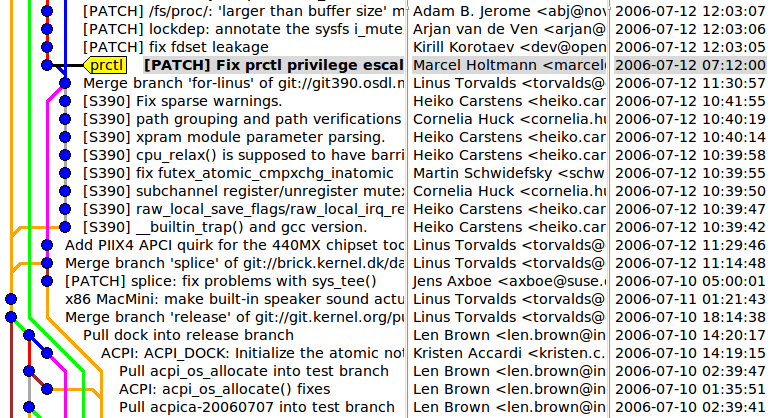
\includegraphics[width=12cm]{prctl}
\end{frame}

\begin{frame}
  \frametitle{A Git repository}
  \begin{itemize}
  \item A Git repository is a collection of
    \emph{refs}---\emph{branches} and \emph{tags}.
  \item A ref is a named mutable pointer to an object (usually a
    commit).
    \begin{itemize}
    \item \texttt{HEAD} $\to$ \texttt{refs/heads/master}
    \item \texttt{refs/heads/master} $\to$ \texttt{commit fec6ed\ldots}
    \item \texttt{refs/heads/ftrace} $\to$ \texttt{commit ce5c1e\ldots}
    \item \texttt{refs/tags/v2.6.8} $\to$ \texttt{commit e8ce2f\ldots}
    \item \texttt{refs/tags/v2.6.27} $\to$ \texttt{tag 4b5127\ldots}
    \end{itemize}
  \item The repository automatically stores the directed acyclic graph
    of objects rooted at these refs.
  \end{itemize}
\end{frame}

\end{document}
